Particle systems can have many different movement mechanisms and the best way to truly understand them is through design and implementation. This is what I did, I designed four different particle systems and packaged their implementations in a simple API for later use. This API (API is the acronym for "Aplication Programming Interface") is designed with extensibility in mind meaning that new particle based graphical effects can be easily added to the next versions of the API.\\

The following particle based graphical effects are offered by the current version of the API:

\begin{itemize}
	\item the conic flame effect.
	
	\item the cylindrical flame effect.
	
	\item the conic flame effect (reversed).
	
	\item the fountain effect.
\end{itemize}

In order to obtain the conic flame effect one must use a particle system in which all the particles are spawned exactly at the tip of an imaginary cone and move towards the base of it.\\

To obtain the cylindrical flame effect one must use a particle system in which all the particles are spawned at one end of an imaginary cylinder and move towards the other end of it.\\

The reversed conic flame effect is basically a conic flame effect in which the particles are spawned at the base of an imaginary cone and move towards the tip of it.

The fountain particle system is somewhat based on the cone shaped particle system. The difference between the two of them is that in the case of the fountain particle system the particles are affected by gravity. In other words the fountain particle system sprays particles exactly like the cone shaped particle system does it only in the case of the fountain particle system the movement of the particle system is curved by a gravity force.\\

The following sections describe exactly how the four particle system types were conceived.\\

\newpage
\section{The Cone Shaped Particle System}
In order for the particle system to look like a cone (it will look roughly like a cone, it will actually have the resemblance of a sprayed flame) all the particles must be spawned exactly at the tip of an imaginary cone and must move towards random points which reside inside an imaginary sphere (the points can also lie on the sphere) which is placed exactly at the base of the cone.\\

\begin{figure}[h]
	\caption{Cone shaped particle system sketch}
	\centering
	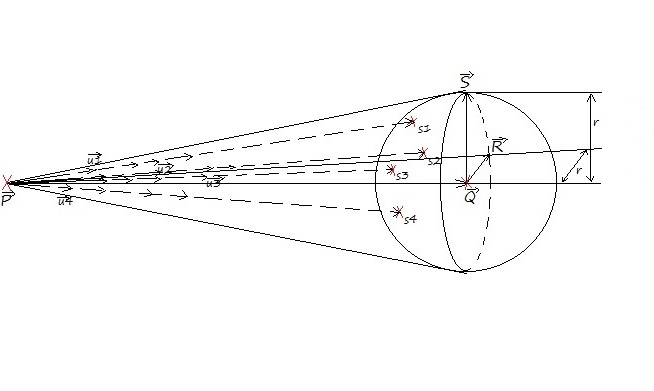
\includegraphics{cone.jpg}
\end{figure}

The sketch from Figure 3.1 shows how to conceive a cone shaped particle system. All the descriptions of the notations from the sketch are given bellow.\\

\begin{itemize}
	\item $\vec{P}$ represents the initial position vector, all the particles will have their position attribute initialized with this vector.
	
	\item $\vec{Q}$ represents the position vector of the center of the sphere. This vector is used to compute the destination position vectors which will lie inside or on the sphere.
	
	\item $\vec{s_1}, \vec{s_2}, \vec{s_3}$ and $\vec{s_4}$ represent the destination position vectors which lie inside or on the sphere.
	
	\item $\vec{u_1}, \vec{u_2}, \vec{u_3}$ and $\vec{u_4}$ represent series of direction vectors. These vectors are used to move each particle from the system in the particle update step. These vectors can be obtained by either normalizing the destination position vectors ($\vec{s_1}, \vec{s_2}$, ...) or by dividing them with a constant meant to scale them down.
	
	\item $r$ represents the size of the radius of the sphere. This radius is also the radius of the circle which forms the base of the cone. The value of this radius is used to compute the destination position vectors ($\vec{s_1}, \vec{s_2}$, ...).
\end{itemize}

For every frame that gets rendered on the screen the following steps are executed:

\begin{enumerate}
	\item Generate a number of particles.
	
	\item Initialize their position attributes with $\vec{P}$ (the position vector which points to the tip of the cone)
	
	\item Generate a set $S = \{\vec{s_1}, \vec{s_2}, \vec{s_3}, \vec{s_4}, ...\}$ of random destination position vectors for each spawned particle which will lie inside or on the sphere with the center in $\vec{Q}$.
	
	\item Use all the previously generated position vectors (from the set $S$) to generate a set $U = \{\vec{u_1}, \vec{u_2}, \vec{u_3}, \vec{u_4}, ...\}$ of direction vectors for each spawned particle.
	
	\item Update the position attribute of each particle from the particle system by simply adding their corresponding direction vector (each particle will have its own $\vec{u}$ from the previously generated set $U$) to their current position vector.
	
	\item Remove all the "dead" particles from the particle system.
	
	\item Render the current image of the particle system.
\end{enumerate}
\newpage
The greatest problem in the rendering process of a cone shaped particle system is how to generate destination position vectors that lie inside or on the surface of an sphere.

The equation of a circle is:
\begin{center}
	$(x - a) ^ 2 + (y - b) ^ 2 = r ^ 2$,
\end{center}

where $a$ and $b$ represent the two-dimensional coordinates of the center of the circle, $r$ represents the radius of the circle and $x$ and $y$ represent the coordinates of all the points on the circle.\\

\begin{figure}[h]
	\caption{Testing the borders of a circle}
	\centering
	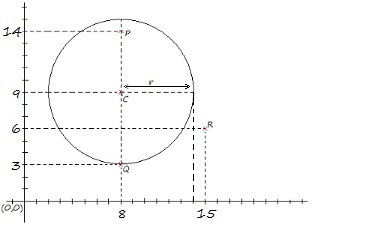
\includegraphics{circle.jpg}
\end{figure}

For example the equation of the circle from Figure 3.2 which has its center positioned in $C\big(8, 9\big)$ and its radius $r = 6$ will look like this:

\begin{center}
	$(x - 8) ^ 2 + (y - 9) ^ 2 = 36$
\end{center}

\newpage
Our concern here is how to generate points that are inside or on the circle with the previously mentioned equation. What we can do is to take three random points, one inside the circle, one exactly on the circle and one outside the circle substitute their coordinates in the equation and see how they verify the equation. Let us take for example $P(8, 14)$, $Q(8, 3)$ and $R(15, 9)$. As you can notice from Figure 3.2 $P$ is inside the circle, $Q$ is exactly on the circle and $R$ is outside the circle.\\

For $P(8, 14)$ we get:
\begin{align*}
	(8 - 8) ^ 2 + (14 - 9) ^ 2 &= 36\\
	0 ^ 2 + 5 ^ 2 &= 36\\
	25 &= 36\ (F)
\end{align*}

For $Q(8, 3)$ we get:
\begin{align*}
(8 - 8) ^ 2 + (3 - 9) ^ 2 &= 36\\
0 ^ 2 + (-6) ^ 2 &= 36\\
36 &= 36\ (T)
\end{align*}

And for $R(15, 9)$ we get:
\begin{align*}
(15 - 8) ^ 2 + (9 - 9) ^ 2 &= 36\\
7 ^ 2 + 0 ^ 2 &= 36\\
49 &= 36\ (F)
\end{align*}

As you can see in the case of $P(8, 14)$ (the point inside the circle) the left side of the equation is smaller than the right side. In the case of $Q(8, 3)$ (the point exactly on the circle) the left side of the equation is equal with the right side and in the case of $R(15, 9)$ (the point outside the circle) the left side of the equation is greater than the right side.\\

From this we can deduce that in order for a point to be inside or on a circle its coordinates must verify the following in-equation:

\begin{center}
	$(x_{point} - x_{circle}) ^ 2 + (y_{point} - y_{circle}) ^ 2 \le r ^ 2$,
\end{center}
where $x_{point}$, $y_{point}$ are the coordinates of the point, $x_{circle}, y_{circle}$ are the coordinates of the center of the circle and r is the radius of the circle.\\

\newpage
If we apply a square root to the both sides of the in-equation we obtain the following:

\begin{center}
	$\sqrt{(x_{point} - x_{circle}) ^ 2 + (y_{point} - y_{circle}) ^ 2} \le r$
\end{center}

We can observe that the left side of the in-equation is actually the formula for computing the distance between two points in space. What this in-equation actually says is that the distance between the center of the circle and any point inside or on the circle must be at most equal with the radius of the circle. This means that we can use the following routine to generate every point inside or on the circle:

\begin{enumerate}
	\item Generate a pair of random values, let us call them $a$ and $b$, from the interval $\big[-r, r\big]$.
	
	\item Compute the coordinates of the randomly generated point (which will never be outside the circle) like this:\\
	$(x_{point}, y_{point}) = (x_{circle}, y_{circle}) + (a, b)$
\end{enumerate}

I used a similar mechanism in the generation of destination position vectors for the cone shaped particle system. Only for the cone shaped particle system I used a sphere instead of a circle. I adapted the previously mentioned routine in order to fit the following in-equation:

\begin{center}
	$\sqrt{(x_{point} - x_{sphere}) ^ 2 + (y_{point} - y_{sphere}) ^ 2 + (z_{point} - z_{sphere}) ^ 2} \le r$
\end{center}